\documentclass[pdftex]{beamer}
%\documentclass[notes=show]{beamer}
%\documentclass[xcolor=dvipsnames]{beamer}

\usepackage{amssymb}
\usepackage{latexsym}
\usepackage{amsfonts}
\usepackage{amsmath}
\usepackage[absolute,overlay]{textpos}
\usepackage[english]{babel}
\usepackage[latin1]{inputenc}
%\usepackage{times}
\usepackage[T1]{fontenc}
\usepackage{tabularx}
\newcolumntype{Y}{>{\small\raggedright\arraybackslash}X}
\usepackage{graphicx}
\usepackage{bigstrut}
\usepackage{bbm}
\usepackage{mathrsfs}
\usepackage{epsfig}
\usepackage{array}
%\usepackage{natbib}

\mode<presentation> {
%\usetheme[left,width=1.7cm]{Berkeley}
%\usetheme{default}
\usetheme{Boadilla}
  \usecolortheme[RGB={103,102,204}]{structure}
%\usecolortheme{dove}
  \useoutertheme{infolines}
  \setbeamercovered{transparent}
 }

%\renewcommand{\familydefault}{cmss}
%\renewcommand{\mathrm}{\mathsf}
%\renewcommand{\textrm}{\textsf}
\usefonttheme{serif}
\newcommand{\X}{{\mathbf{X}}}
\newcommand{\x}{{\mathbf{x}}}
\newcommand{\E}{\mathsf{E}}
\newcommand{\V}{\mathsf{Var}}

\DeclareGraphicsExtensions{.jpg,.pdf,.mps,.png}

    %%%%%%%%%%%%%%%%%%%%%%%%%%%%%%%%%%%%%%%%%%%%%%%%%%%%%%%%%%%%%%%%%%%%%%%%%%%%%%
    %         Neue Kommandos f�r fette Mathebuchstaben innerhalb von Formeln     %
    %%%%%%%%%%%%%%%%%%%%%%%%%%%%%%%%%%%%%%%%%%%%%%%%%%%%%%%%%%%%%%%%%%%%%%%%%%%%%%
    \newcommand{\bom}{\boldmath}
    \newcommand{\ubom}{\unboldmath}
    \newcommand{\mb}{\mathbf}

    \newcommand{\fmalpha}{\mbox{\bom${\alpha}$}}               %Fettes alpha
    \newcommand{\fmbeta}{\mbox{\bom${\beta}$}}                 %Fettes beta
    \newcommand{\fmgamma}{\mbox{\bom${\gamma}$}}               %Fettes gamma
    \newcommand{\fmdelta}{\mbox{\bom${\delta}$}}               %Fettes delta
    \newcommand{\fmepsilon}{\mbox{\bom${\epsilon}$}}           %Fettes epsilon
    \newcommand{\fmvarepsilon}{\mbox{\bom${\varepsilon}$}}     %Fettes varepsilon
    \newcommand{\fmzeta}{\mbox{\bom${\zeta}$}}                 %Fettes zeta
    \newcommand{\fmeta}{\mbox{\bom${\eta}$}}                   %Fettes eta
    \newcommand{\fmta}{\mbox{\bom${\theta}$}}                  %Fettes theta (ta)
    \newcommand{\fmvarta}{\mbox{\bom${\vartheta}$}}         	 %Fettes vartheta (ta)
    \newcommand{\fmiota}{\mbox{\bom${\iota}$}}                 %Fettes iota
    \newcommand{\fmkappa}{\mbox{\bom${\kappa}$}}               %Fettes kappa
    \newcommand{\fmla}{\mbox{\bom${\la}$}}                     %Fettes lambda (la)
    \newcommand{\fmmu}{\mbox{\bom${\mu}$}}                     %Fettes mu
    \newcommand{\fmnu}{\mbox{\bom${\nu}$}}                     %Fettes nu
    \newcommand{\fmxi}{\mbox{\bom${\xi}$}}                     %Fettes xi
    \newcommand{\fmo}{\mbox{\bom${\o}$}}                       %Fettes o
    \newcommand{\fmpi}{\mbox{\bom${\pi}$}}                     %Fettes pi
    \newcommand{\fmPi}{\mbox{\bom${\Pi}$}}                     %Fettes pi
    \newcommand{\fmvarpi}{\mbox{\bom${\varpi}$}}               %Fettes varpi
    \newcommand{\fmrho}{\mbox{\bom${\rho}$}}                   %Fettes rho
    \newcommand{\fmvarrho}{\mbox{\bom${\varrho}$}}             %Fettes varrho
    \newcommand{\fmsigma}{\mbox{\bom${\sigma}$}}               %Fettes sigma
    \newcommand{\fmSigma}{\mbox{\bom${\Sigma}$}}               %Fettes sigma
    \newcommand{\fmvarsigma}{\mbox{\bom${\varsigma}$}}         %Fettes varsigma
    \newcommand{\fmtau}{\mbox{\bom${\tau}$}}                   %Fettes tau
    \newcommand{\fmupsilon}{\mbox{\bom${\upsilon}$}}           %Fettes upsilon
    \newcommand{\fmphi}{\mbox{\bom${\phi}$}}                   %Fettes phi
    \newcommand{\fmvarphi}{\mbox{\bom${\varphi}$}}             %Fettes varphi
    \newcommand{\fmchi}{\mbox{\bom${\chi}$}}                   %Fettes chi
    \newcommand{\fmpsi}{\mbox{\bom${\psi}$}}                   %Fettes psi
    \newcommand{\fmomega}{\mbox{\bom${\omega}$}}               %Fettes omega
    \newcommand{\fmimath}{\mbox{\bom${\imath}$}}               %Fettes imath
    \newcommand{\fmOmega}{\mbox{\bom${\Omega}$}}                     %Fettes Omega


\setbeamercolor{bibliography entry title}{fg=black}
\setbeamercolor{bibliography entry author}{fg=black}
\setbeamercolor{subsection in toc}{fg=structure}
\setbeamercolor{palette primary}{bg=structure, fg=white}
%\setbeamercolor{palette secondary}{bg=structure, fg=black}
%\setbeamercolor{palette tertiary}{bg=structure, fg=black}
\setbeamercolor{caption name}{fg=black} \setbeamersize{text margin
left=.8cm} \setbeamersize{text margin right=1cm}
\hypersetup{linkbordercolor={1 0 0}} \setbeamertemplate{navigation
symbols}{} \setbeamertemplate{headline}[default]

\setbeamertemplate{enumerate items}[default]

\newcounter{transfct}
\newcounter{begbs}
\newcounter{endbs}


\title[Fuzzy Regression Discontinuity]{Econometrics 2 (Part 1)}

\author[Lychagin  \& Mu\c co]{Arieda Mu\c co}
\institute[CEU]{Central European University}
\date{Spring 2020}

\AtBeginSection[] {
  \begin{frame}<handout:0>
    \frametitle{TOC}
    \tableofcontents[currentsection]
  \end{frame}
}


\AtBeginSection[] {
  \begin{frame}<handout:0>
    \frametitle{TOC}
    \tableofcontents[currentsection]
  \end{frame}
}


\pgfdeclareimage[height=.7cm]{logo}{rgs2}
\logo{\pgfuseimage{logo}}
\begin{document}

\frame{\titlepage}

%%%%%%%%%%%%%%%%%%%%%%%%%%%%%%%%%%%%%%%%%%%



\frame{ \frametitle{Fuzzy Regression Discontinuity}

Probability of receiving treatment does not change from 0 to one at the cutoff, but

\begin{equation*}
\underset{z\uparrow z_0}{lim} P(D_i=1|z_i=z) \neq \underset{z \downarrow z_0}{lim} P(D_i=1|z_i=z)
\end{equation*}
other variables also determine treatment assignment, but incentives to participate change discontinuously at the threshold.
\begin{itemize}

\item Examples: Incentives to participate in some program may change discontinuously at
the cutoff but are not powerful enough to move everyone from non participation to
participation.
\end{itemize}

}
%---------------------------------------------------------------------------------%
 \frame{ \frametitle{Example}
\begin{center}
\begin{figure}[t]
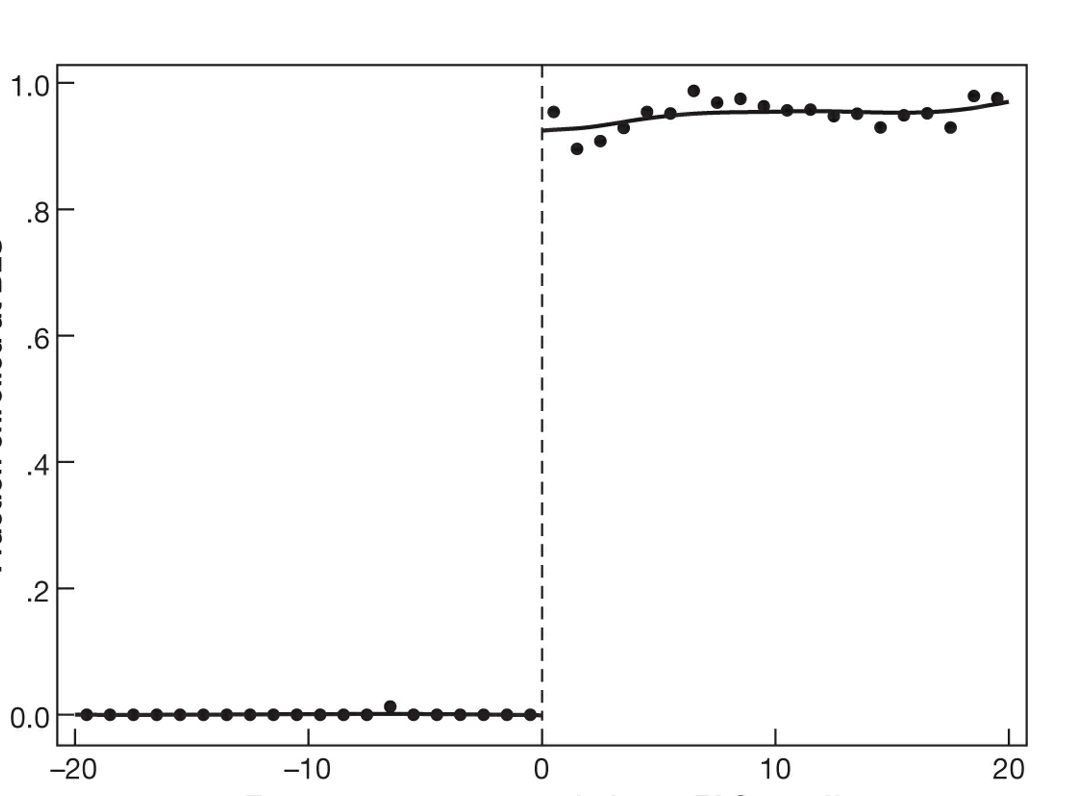
\includegraphics[scale=.50]{graphs/Example_fuzzy.png}
\end{figure}
\end{center}
 }
%---------------------------------------------------------------------------------%

\frame{ \frametitle{Fuzzy Regression Discontinuity is IV}
\begin{equation*}
      \hat{\rho}_{f}= \frac{\underset{z \downarrow z_0}{lim} E(Y_i|z_i=z) -\underset{z\uparrow z_0}{lim} E(Y_i|z_i=z)}
     {\underset{z \downarrow z_0}{lim} E(D_i|z_i=z) -\underset{z\uparrow z_0}{lim} E(D_i|z_i=z)}
\end{equation*}
Fuzzy RD is numerically equivalent and conceptually similar to instrumental
variables

\begin{itemize}
  \item Numerator: "jump" in the regression of the outcome on the running variable, $z$.
\textbf{Reduced form}
  \item Denominator: "jump" in the regression of the treatment indicator on the running
variable $z$. \textbf{First stage}
\end{itemize}
Idea: use the discontinuity created by this rule to identify the treatment effect

 }
%---------------------------------------------------------------------------------%
\frame{ \frametitle{First stage relationship between $Z$ and D}
\begin{itemize}
  \item In the sharp RD, $D_i$ was determined by $z_i$  and  $z_0$; in the fuzzy RD, the
conditional probability of treatment jumps at $z_0$
  \item The relationship between the probability of treatment and $z_i$ can be written as:
\begin{equation*}
P(D_i=1|z_i)=E(D_i=1|z_i)=g_0(z_i)+[ g_0(z_i)-g_1(z_i)]T_i
\end{equation*}
\item where $T_i= 1$ if $(z_i \geq z_0)$ and 0 otherwise; indicating the point of discontinuity in $E (D_i=1|z_i)$
\end{itemize}

}

%---------------------------------------------------------------------------------%


  \frame{ \frametitle{Fuzzy design}
\begin{center}
\begin{figure}[t]
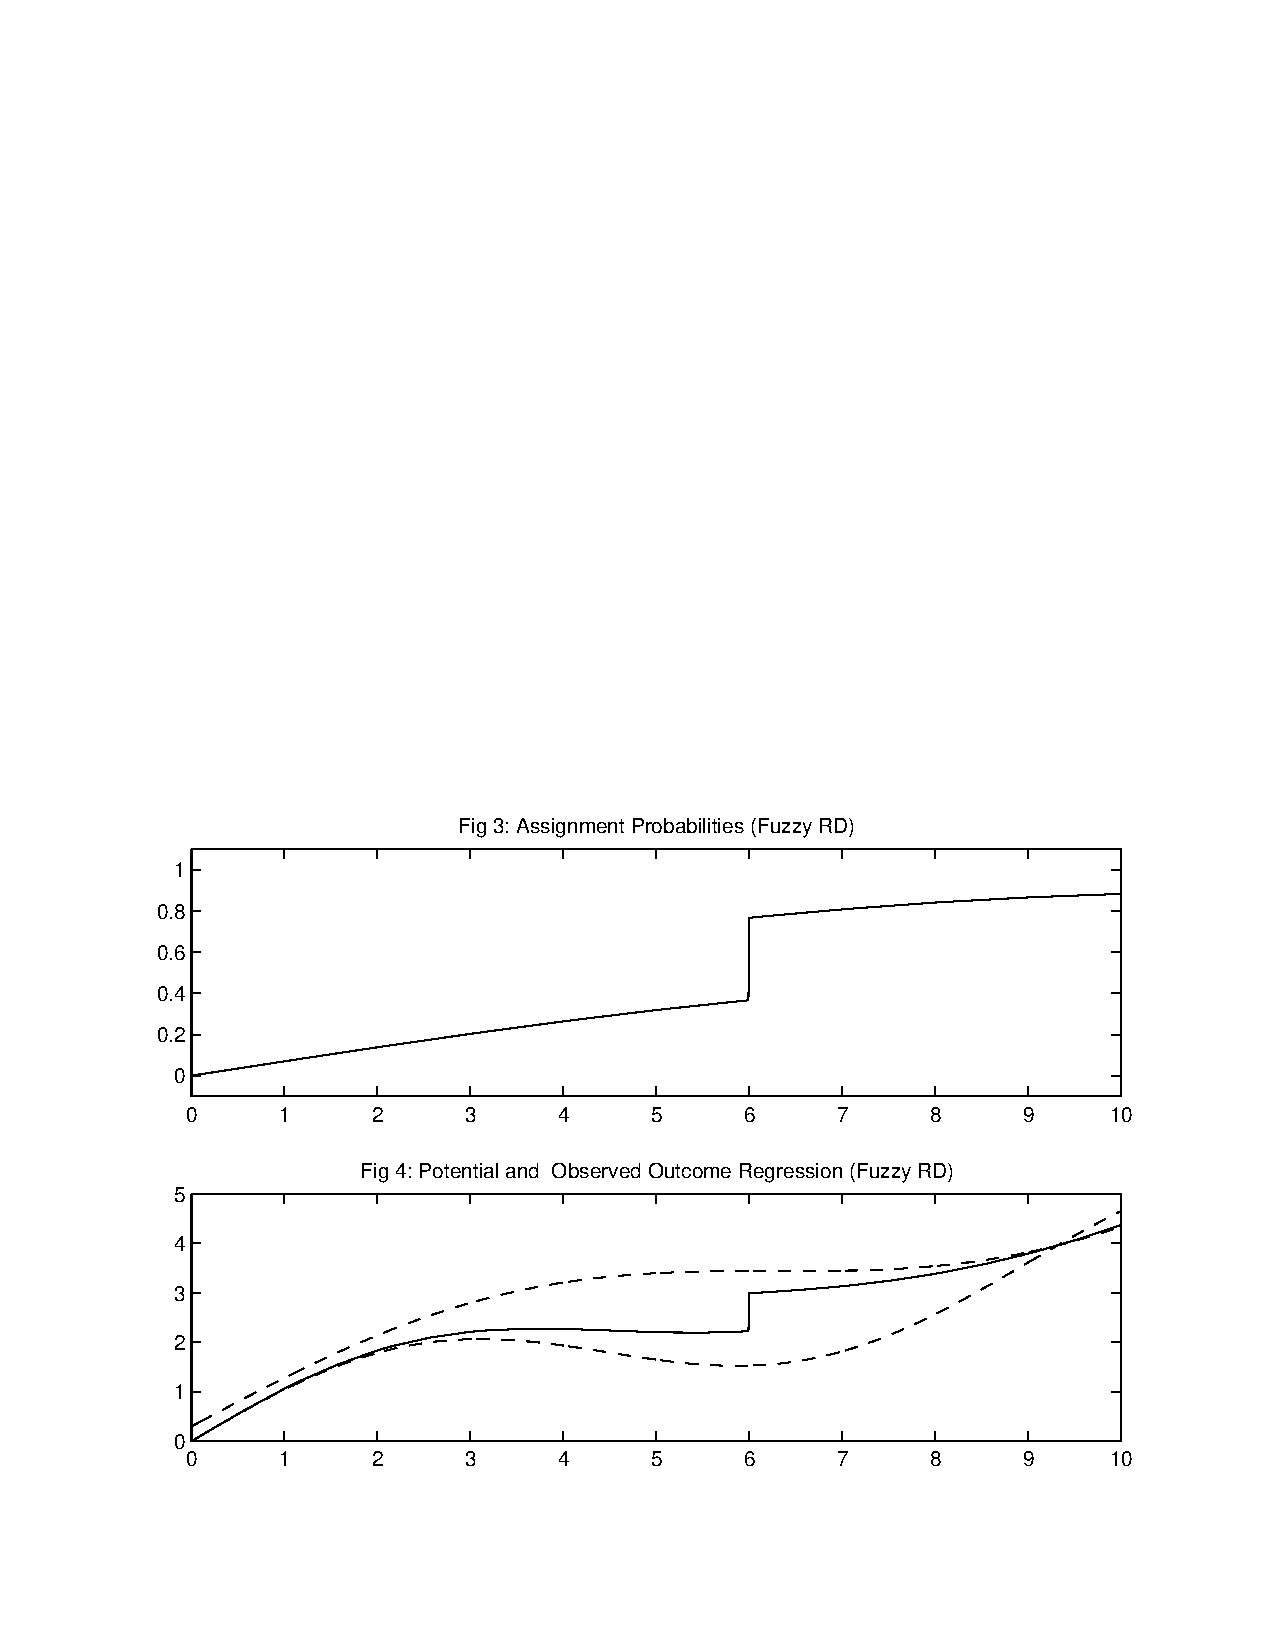
\includegraphics[scale=.60]{graphs/imbens_lemieux_fig2.pdf}
\end{figure}
\end{center}
 }

%---------------------------------------------------------------------------------%
\frame{ \frametitle{First stage relationship between $Z$ and D}
\begin{itemize}
  \item One can use both  $T_i$ as well as the interaction terms as instruments for $D_i$.
  \item The  first stage would be:
\begin{equation*}
D_i=\gamma_0 +\gamma_1 z_i +\gamma_2 z_i^2  +\gamma_3 z_i^3+...+\gamma_p z_i^p+ \pi T_i + \zeta_{1i}
\end{equation*}
\item where $\pi$ is the causal effect of $T_i$ on the conditional probability of treatment
\item The fuzzy RD reduced form is:
\begin{equation*}
Y_i= \mu+\kappa_1 z_i +\kappa_2 z_i^2  +\kappa_3 z_i^3+... +\kappa_p z_i^p+ \rho \pi T_i + \zeta_{2i}
\end{equation*}
 \end{itemize}
 
 
}


%---------------------------------------------------------------------------------%

 \frame{ \frametitle{Fuzzy RD with varying Treatment Effects - Second Stage}
\begin{itemize}

\item As in the sharp RD case one can allow the smooth function
to be different on both sides of the discontinuity
\item The second stage model with interaction terms would be the
similar to before:
\end{itemize}
\begin{equation*}
\begin{aligned}
    Y_i= \alpha+\beta_{01} \tilde{z_i} +\beta_{02} \tilde{z_i} ^2  +\beta_{03} \tilde{z_i} ^3+... +\beta_{0p}  \tilde{z_i} ^p 
    \\
     +\rho D_i+ \beta^{*}_{1}D_i \tilde{z_i} +\beta^{*}_{2}D_i \tilde{z_i} ^2  +\beta^{*}_{3} D_i \tilde{z_i}^3+... +\beta^{*}_{p}D_i\tilde{z_i}^p+ \eta_{i}
\end{aligned}
\end{equation*}
Where $\tilde{z_i} $ are now not only normalized with respect to ${z_0}$ (also fitted values obtained from the first stage regression)

 }
 %---------------------------------------------------------------------------------%

  \frame{ \frametitle{Fuzzy RD with varying Treatment Effects - First Stage}
\begin{itemize}

\item Again one can use both $T_i$ as well as the interaction terms as
instruments for $D_i$
\item Only using T the estimated  first stages would be:
\end{itemize}
\begin{equation*}
\begin{aligned}
D_i=\gamma_{00} +\gamma_{01} \tilde{z_i} +\gamma_2 \tilde{z_i}^2  +\gamma_3 \tilde{z_i}^3+...+\gamma_p \tilde{z_i}^p+ \\
     +\pi  T_i + \gamma^{*}_{1}T_i \tilde{z_i} +\gamma^{*}_{2}T_i \tilde{z_i}^2  +\gamma^{*}_{3} T_i \tilde{z_i}^3+... +\gamma^{*}_{p}T_i\tilde{z_i}^p+ \eta_{i}
\end{aligned}
\end{equation*}
 }
%---------------------------------------------------------------------------------%

 \frame{ \frametitle{What does Fuzzy RDD Estimate?}
\begin{itemize}

\item As Hahn, Todd and van der Klaauw (2001) point out, one
needs the same assumptions as in the standard IV framework
 
\item As with other binary IVs, the fuzzy RD is estimating LATE:
the average treatment effect for the compliers
\item In RD, the compliers are those whose treatment status
changed as we moved the value of $z_i$ from just to the left of
$z_0$ to just to the right of $z_0$
\end{itemize}
 }
 %---------------------------------------------------------------------------------%

 \title[Regression Discontinuity]{Econometrics 2 (Part 1)}

 \frame{ \frametitle{Challenges to RD (not only Fuzzy)}
\begin{itemize}

\item Treatment is not as good as randomly assigned around the cutoff, $z_0$, when
agents are able to manipulate their running variable scores. This happens
when:
 \begin{enumerate}
\item The assignment rule is known in advance
\item  Agents are interested in adjusting
\item Agents have time to adjust
 \end{enumerate}
\item \textbf{Examples:} re-take an exam, self-reported income, etc.


\item Some other unobservable characteristic changes at the threshold, and this has a
direct effect on the outcome.
\item In other words, the cutoff is endogenous
\item \textbf{Example:} Age thresholds used for policy (i.e., person turns 18, and faces more
severe penalties for crime) is correlated with other variables that affect the outcome (i.e., graduation, voting rights, etc.)
\end{itemize}

Several formalized tests to evaluate the severity of these problems...
 }
 
  %---------------------------------------------------------------------------------%

 \frame{\frametitle{Manipulation of the running variable}
 Sorting on the running variable
\begin{itemize}
\item Assume a treatment, D, is assigned by rule $z  \geq z_0$, if individuals chose $z$ such that they sort into D then we say individuals are sorting on
the running variable
\item \textbf{Example:}  Suppose a doctor plans to randomly assign heart patients to a medicine that lowers cholesterol and a placebo to study the effect of the medicine on heart attacks
within 10 years. The doctor randomly assigns patients to two different waiting
rooms, A and B, and plans to give those in A the medicine and those in B the
placebo. If some of the patents learn of the planned treatment assignment
mechanism, what would we expect to happen? And how would you check for
it?
\end{itemize}
 }
 
 %---------------------------------------------------------------------------------%

  \frame{\frametitle{McCrary Density Test}
 Sorting on the running variable
\begin{itemize}
\item We would expect waiting room A to become crowded. In the RDD context, sorting
on the running variable implies heaping on the "good side" of $z_0$
the running variable
\item McCrary (2008) suggests a formal test. Under the null the density should be
continuous at the cutoff point. Under the alternative hypothesis, the density
should increase at the cutoff (where D is viewed as good)
 \begin{enumerate}
\item Partition the assignment variable into bins and calculate frequencies (i.e., number
of observations) in each bin
\item  Treat those frequency counts as dependent variable in a local linear regression
 \end{enumerate}
\end{itemize}
 }
 %---------------------------------------------------------------------------------%

   \frame{\frametitle{McCrary Density Test}
 The McCrary Density Test has become mandatory for every analysis using
RD
\begin{itemize}
\item If you can estimate the conditional expectations, with data on the
running variable. In principle you can always do a density test
\item For RD to be useful, you already need to know something about the
mechanism generating the assignment variable and how susceptible it could be
to manipulation. Note the rationality of economic actors that this test is built
on
\item A discontinuity in the density is "suspicious"  it suggests manipulation is probably going on.
This is a high-powered test. You need a lot of observations at $z_0$ to distinguish a discontinuity in the density from noise
\end{itemize}
 }
 %---------------------------------------------------------------------------------%

    \frame{ \frametitle{McCrary Density Test}
\begin{center}
\begin{figure}[t]
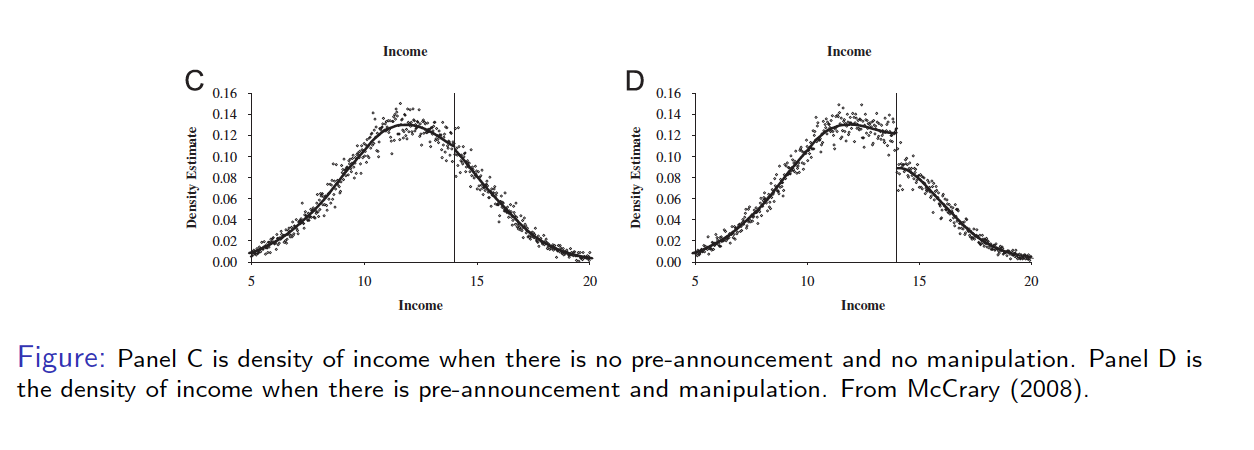
\includegraphics[scale=.50]{graphs/mcrary.png}
\end{figure}
\end{center}
 }
 
 %---------------------------------------------------------------------------------%

    \frame{\frametitle{Lee (2008) Incumbency Effect}
\begin{itemize}
\item David Lee (2008) "Randomized Experiments from non-random selection in
US House Elections", Journal of Econometrics analyzes the incumbency effect using Democratic incumbents for US congressional elections
\item A large political science literature on the "incumbency advantage"  having won
an election once helps you win subsequent elections.
\item Empirical challenge: how to separate incumbency advantage from selection? 
(i.e., candidates win multiple elections because they are better)


\end{itemize}
}
%---------------------------------------------------------------------------------%


\frame{\frametitle{Lee (2008) Incumbency Effect}

\begin{itemize}
\item Identification: Incumbency is assigned to a candidate discontinuously at 50\% voteshare under two-party democracy with majority rule
\item Lee (2008) analyzes the probability of winning the election in year $t + 1$ by
comparing candidates who just won to candidates who just lost the election in
year $t$.
\end{itemize}
\begin{center}
\begin{figure}[t]
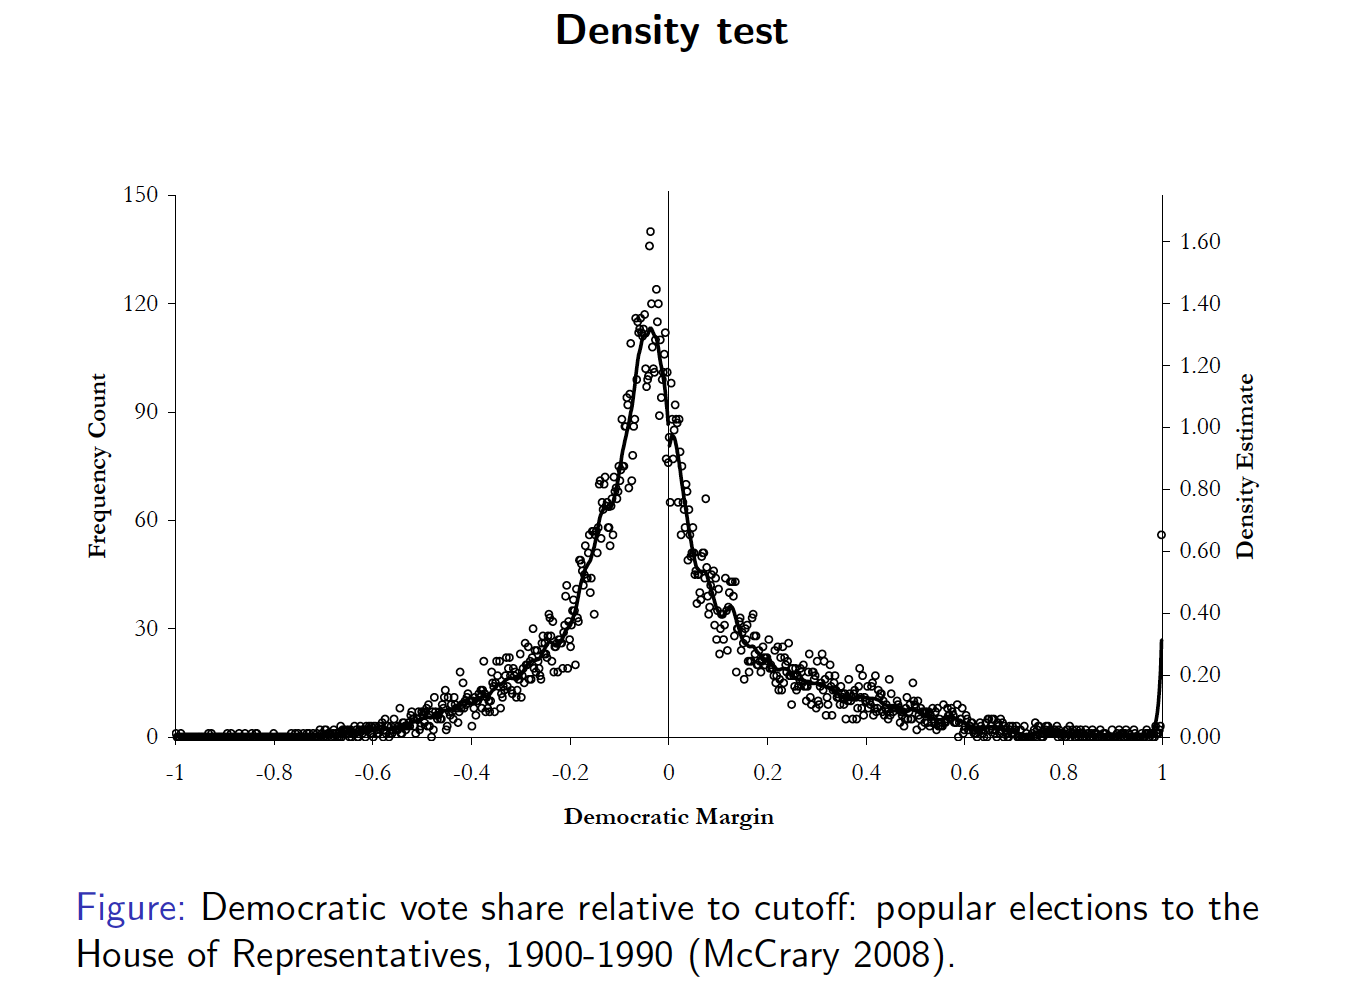
\includegraphics[scale=.30]{graphs/lee_vs1.png}
\end{figure}
\end{center}
 }
 %---------------------------------------------------------------------------------%


 \frame{\frametitle{More evidence of manipulation}

\begin{itemize}
\item Contrast this with roll call voting in the US House of Representatives
\item Coordination is expected because these are repeated games, votes are public
records, and side payments are possible in the form of future votes
\item Bills around the cutoff are more likely to be passed than not. Seems like a good
candidate for RD
\item Fails McCrary Density Test; cannot use RD because policy decisions are not
quasi-randomly assigned at the cutoff 
\end{itemize}
\begin{center}
\begin{figure}[t]
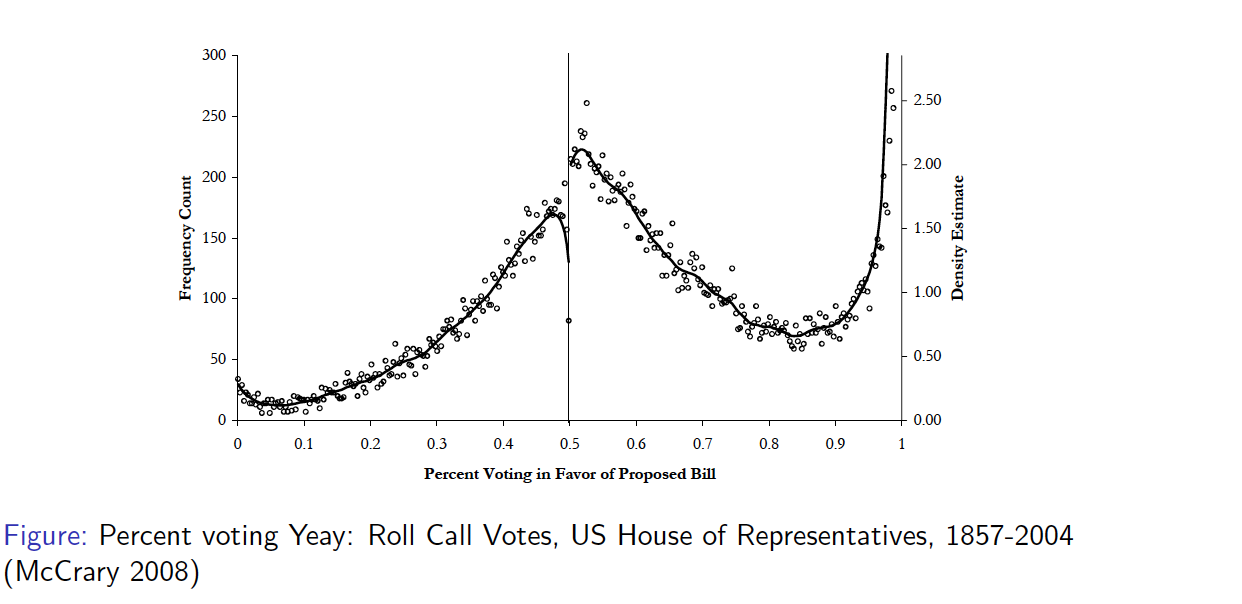
\includegraphics[scale=.30]{graphs/lee_vs2.png}
\end{figure}
\end{center}
 }
 %---------------------------------------------------------------------------------%

\frame{\frametitle{Balance test on covariates}

\begin{itemize}
\item This is a type of placebo test. For RD to be valid in your
study, you do not want to observe a discontinuity around the
cutoff, $z_0$, for average values of covariates that should not be
affected by the treatment ( e.g., pretreatment characteristics)
\item Question: What does a jump in the average values of
pre-treatment characteristics have to do with the continuous
(smoothness) assumption?
\begin{itemize}
\item Choose pre-treatment covariates, $X$, and do a similar
graphical plot as you did for Y
\item You \textbf{do not want} to see a jump around the cutoff, $z_0$
\item A formal balance test involves the same procedure used to
estimate the treatment effect, only use $X$ instead of $Y$ as a
LHS variable
\item Can combine test on multiple covariates into a single test
\end{itemize}
\end{itemize}
 }
 %---------------------------------------------------------------------------------%

 \frame{\frametitle{Visualizing Balanced Placebos}
 \begin{center}
\begin{figure}[t]
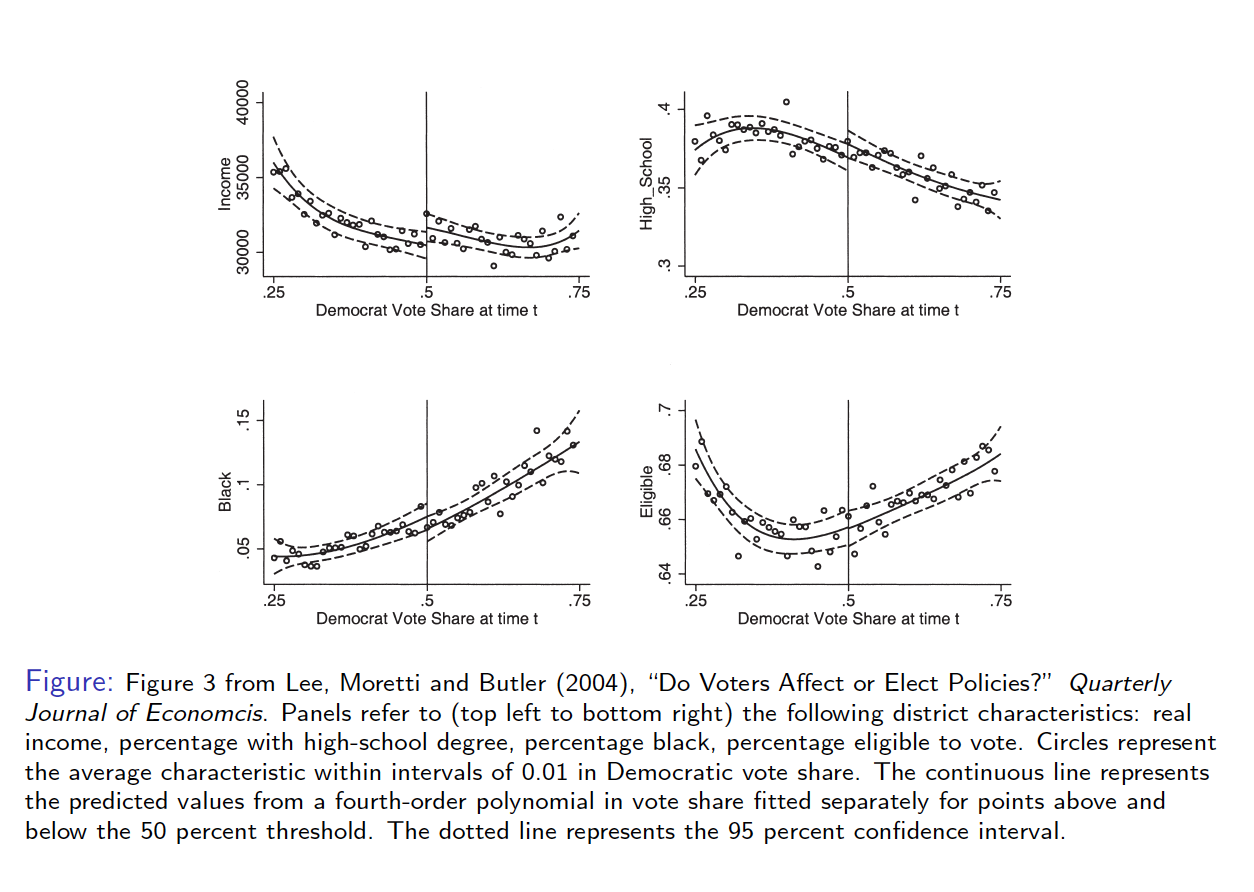
\includegraphics[scale=.50]{graphs/visualizing_placebos.png}
\end{figure}
\end{center}
 }
%---------------------------------------------------------------------------------%
 
  \frame{\frametitle{Jumps at non-discontinuous points}
\begin{itemize}
\item Imbens and Lemieux (2008) suggest to look at one side of the
discontinuity (e.g., $z < z_0$), take the median value of the
running variable in that section, and pretend it was a
discontinuity
\item Then test whether in reality there is a discontinuity at ${z_0}^{'}$. You do not want to find anything
\item Look for non-effects in non-treatment periods
\end{itemize}
 }
 %---------------------------------------------------------------------------------%

  \frame{\frametitle{Examples Fuzzy RD}
\begin{itemize}
\item  Tyrefors Hinnerich and Pettersson-Lidbom, Econometrica(2014)
\item Does the form of Democracy matter?
\item The elite can capture democratic political process by
exercising their de facto political power
\begin{itemize}
\item Lack of (pro-poor) political parties in direct democracy
made it harder for the citizens to solve their collective
action problem
\item The chairman of the town meeting has agenda setting
power
\item Elite relies on intimidation
\end{itemize}

\end{itemize}
 }
 
 
   \frame{\frametitle{Tyrefors Hinnerich and Pettersson-Lidbom(2014)}
\begin{itemize}
\item Local Government Act (LGA) of 1863 granted local
governments independent income taxation rights
\item The bulk of local government revenues was still is raised through a local
proportional income tax
\item Focus on rural municipalities (Provide important public services such as education and
social welfare)
\item In 1918, local governments with a population of more than 1,500
people were required by national law to have representative those with population below  could have 1,500 direct democracy
\item If a local government had switched to a representative system, it
could not switch back within a five-year period
democracy 
\item Running variables: Population in 1918 and Population in the year t-1 for the period from 1919
\end{itemize}
 }
 
 
    \frame{\frametitle{Data}
\begin{itemize}
\item Panel dataset for about 2,500 local governments for
the period 1918-1938
\item Published and unpublished material produced by Statistics
Sweden
\item National Archives of Sweden and was collected by hand. For
the published material, we have digitized it by using data-entry
services in India
\item Swedish State church kept vital statistics until 1991
\item Local governments could try to control individuals in and out
\item No evidence of sorting around the threshold
\end{itemize}
 }
 
     \frame{\frametitle{Estimation}
\begin{itemize}
\item Let be the running variable $z_i$, population in local government
(either population size in year $t-1$ or population size in
1918)
\item The local polynomial regression, equivalent to the OLS
estimation using only observations around the cut-off
\[
Y_i= \alpha +\beta D_i +f(z_i)+u_i
\]
\item where $D_i =1$ if local government has direct democracy
\item $\beta $  measures the effect of having direct rather than representative
democracy
\item The eligibility rule $T = 1$ if $z_i \leq 1500$ as an instrument for
treatment status
\end{itemize}
 }
 
 \frame{\frametitle{}
 \begin{center}
\begin{figure}[t]
\includegraphics[scale=.49]{../../../Empirical_Political_course/Slides2019/Images/ppl_tab2.png}
\end{figure}
\end{center}
 }
 
 
 
 \frame{\frametitle{Reduced Form}
 \begin{center}
\begin{figure}[t]
\includegraphics[scale=.55]{../../../Empirical_Political_course/Slides2019/Images/ppl_fig1.png}
\end{figure}
\end{center}
 }
 
 \frame{\frametitle{First Stage}
 \begin{center}
\begin{figure}[t]
\includegraphics[scale=.55]{../../../Empirical_Political_course/Slides2019/Images/ppl_fig2.png}
\end{figure}
\end{center}
 }
 

   \frame{\frametitle{Wald Estimator}
 \begin{center}
\begin{figure}[t]
\includegraphics[scale=.45]{../../../Empirical_Political_course/Slides2019/Images/ppl_tab5.png}
\end{figure}
\end{center}
 }
 
 
 
 \frame{\frametitle{McRary Test}
 \begin{center}
\begin{figure}[t]
\includegraphics[scale=.50]{../../../Empirical_Political_course/Slides2019/Images/ppl_fig3.png}
\end{figure}
\end{center}
 }
 
 
 \end{document}






